\documentclass[10pt,a4paper]{article}
\usepackage[utf8]{inputenc}
\usepackage{amsmath}
\usepackage{dsfont}
\usepackage{amsfonts}
\usepackage{amssymb}
\usepackage{graphicx}

\author{Leander van Beek}
\title{Highly divisible triangular number}

\newcommand{\desda}{\textbf{if and only if} }

\begin{document}

\maketitle

\textbf{Problem 15:} \\
Starting in the top left corner of a 2×2 grid, and only being able to move to the right and down, there are exactly 6 routes to the bottom right corner.\\

\begin{figure}[h]
	\centering
	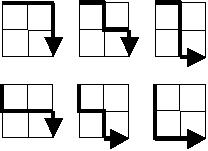
\includegraphics[width=0.4\linewidth]{problem.png}
\end{figure}

How many such routes are there through a 20×20 grid?

\vspace{0.5cm}
\hrule
\vspace{0.5cm}

\section{Solution}

As we are working on a Manhattan metric, all trajectories with the given constraints from A to B are equidistant. The length of the trajectory is the distance that has to be travelled vertically plus the distance that has to be travelled vertically. This means that for the solution, all routes can be described by a combination of 40 characters: D for going downwards and R for going right. Let us describe all routes for the example given above:

\begin{itemize}
	\itemsep0em
	\item RRDD
	\item RDRD
	\item RDDR
	\item DRRD
	\item DRDR
	\item DDRR
\end{itemize}

It can be observed that this is the exhaustive list of unique permutations of 2 R's and 2 D's. To find the number of trajectories, find the number of permutations of this string. The total number of permutations for our problem is found by multiplying the number of possibilities for each element. In the first character, we still have 20 R's and 20D's to pick from. In the second position, we still have 19 of one and still 20 of the other, so 39 in total.  The total number of permutations will then be $40!$.\\
However, exchanging any two R's or D's will give us the same result, so we need to factor out these options. The same strategy can be employed for finding the amount of combinations we can make putting all R's in different positions: this will end up being $20!$ different posibilities. Of course, this is the same for the $D's$, and the total exchange options is then $\left(20!\right)^2$.\\
The final number of trajectories that can be drawn is therefore

\begin{equation}
	\boxed{N = \frac{40!}{\left(20!\right)^2} = 137\ 846\ 528\ 820}
\end{equation}
The solution can be generalized to a non-square rectangular as well: given height H and width L, the number of trajectories is 
\begin{equation}
	\boxed{N = \frac{\left(H \times L\right)!}{H!L!}}
\end{equation}
\end{document}